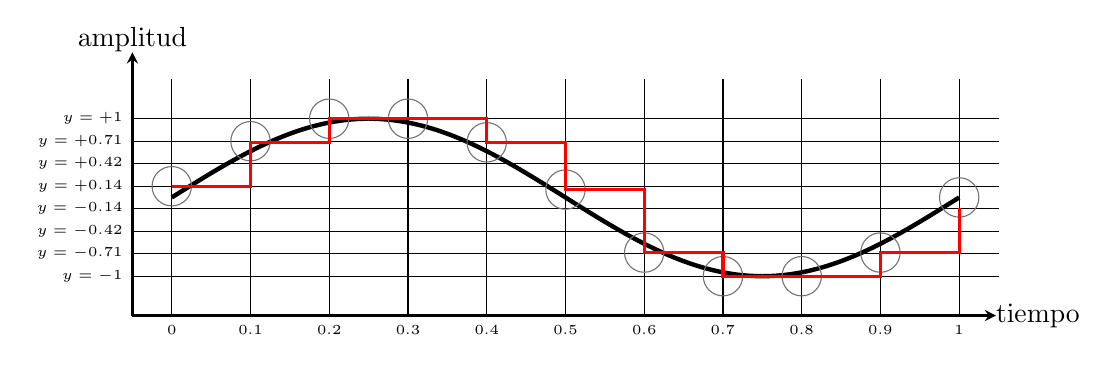
\begin{tikzpicture}
\tikzstyle{stealth} = [-stealth, thick]
\tikzstyle{invisible} = [outer sep=0,inner sep=0,minimum size=0]
\tikzstyle{circle} = [shape=circle, minimum size=0.5cm, draw=black!55]
\tikzstyle{line} = [draw, very thick, red]
    \draw (-0.5,1)node[left,font=\tiny] {$y=+1$} -- (10.5,1);
    \draw (-0.5,0.7142)node[left,font=\tiny] {$y=+0.71$} -- (10.5,0.7142);
    \draw (-0.5,0.4285)node[left,font=\tiny] {$y=+0.42$} -- (10.5,0.4285);
    \draw (-0.5,0.1428)node[left,font=\tiny] {$y=+0.14$} -- (10.5,0.1428);
    \draw (-0.5,-0.1428)node[left,font=\tiny] {$y=-0.14$} -- (10.5,-0.1428);
    \draw (-0.5,-0.4285)node[left,font=\tiny] {$y=-0.42$} -- (10.5,-0.4285);
    \draw (-0.5,-0.7142)node[left,font=\tiny] {$y=-0.71$} -- (10.5,-0.7142);
    \draw (-0.5,-1)node[left,font=\tiny] {$y=-1$} -- (10.5,-1);
    \foreach \x in {0,0.1,0.2,0.3,0.4,0.5,0.6,0.7,0.8,0.9,1}
    {
    	\draw (\x*10,-1.5)node [below,font=\tiny,] {\x } -- (\x*10,1.5) ;
    }
    \draw[ultra thick, ] (0,0) node (v5) {} sin (2.5,1) node (v7) {};
    \draw[ultra thick, ] (2.5,1) cos (5,0) node (v9) {};
    \draw[ultra thick, ] (5,0) sin (7.5,-1) node (v11) {};
    \draw[ultra thick, ] (7.5,-1) cos (10,0) node (v13) {};

\node [invisible] (v1) at (-0.5,-1.5) {};
\node [invisible] (v2) at (-0.5,2) {amplitud};
\node [invisible] (v3) at (11,-1.5) {tiempo};
\draw [stealth] (v1) edge (v2);
\draw [stealth] (v1) edge (v3);
\node [circle] (v4) at (0,0.1428) {};
\node [circle] (v6) at (1,0.7142) {};
\node [circle] (v8) at (2,1) {};
\node [circle] (v10) at (3,1) {};
\node [circle] (v12) at (4,0.7) {};
\node [circle] (v14) at (5,0.1) {};
\node [circle] at (6,-0.7) {};
\node [circle] (v15) at (7,-1) {};
\node [circle] at (8,-1) {};
\node [circle] (v16) at (9,-0.7) {};
\node [circle] (v17) at (10,0) {};
\draw [line](0,0.1428) -- (1,0.1428) node [invisible] {} -- (1,0.7) -- 
			(2,0.7) node [invisible] {} -- (2,1) -- 
			(4,1) node [invisible] {} -- (4,0.7) -- 
			(5,0.7) node [invisible] {} -- (5,0.1) node [invisible] {} --
			(6,0.1) -- (6,-0.7) node [invisible] {} --
			(7,-0.7) node [invisible] {} -- (7,-1) -- 
			(9,-1) node [invisible] {} -- (9,-0.7) -- (10,-0.7) -- (10,-0.14);
\end{tikzpicture}